\section{Context Viewpoint}
\subsection*{View: \textless{}Name\textgreater{}}
\subsubsection*{Model}
Place here the model representation of the view
\begin{figure}[ht]
    \centering
    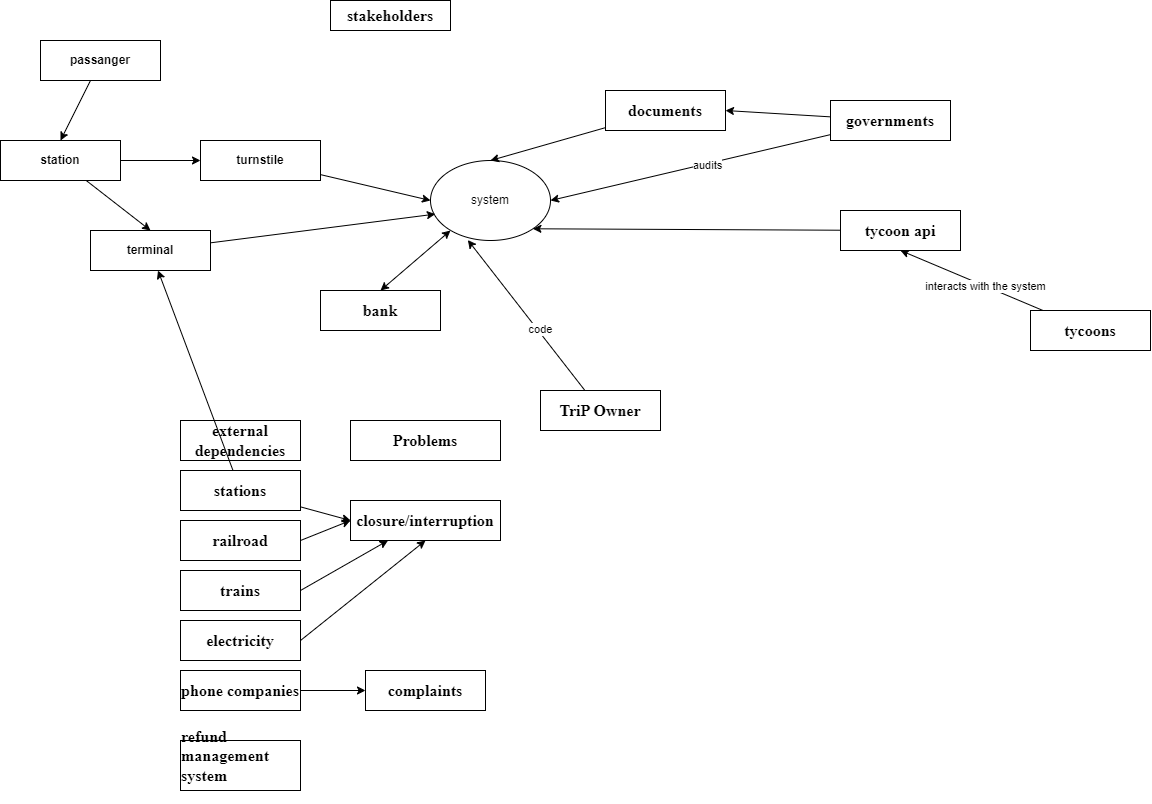
\includegraphics[width=\textwidth]{drawings/views_draft1/context_view_draft1.png}
    \caption{Context view model.}
    \label{fig:context_view_model}
\end{figure}

\subsubsection*{Description}
TODO: Short description of the view

\subsubsection*{Glossary of Elements}
\begin{longtable}{lll}
Id & Name & Description \\
\end{longtable}

\subsection*{Analysis on Perspectives}
Describe how the view satisfies the different perspectives. 

\section{Functional Viewpoint}
\begin{figure}[h!]
    \centering
    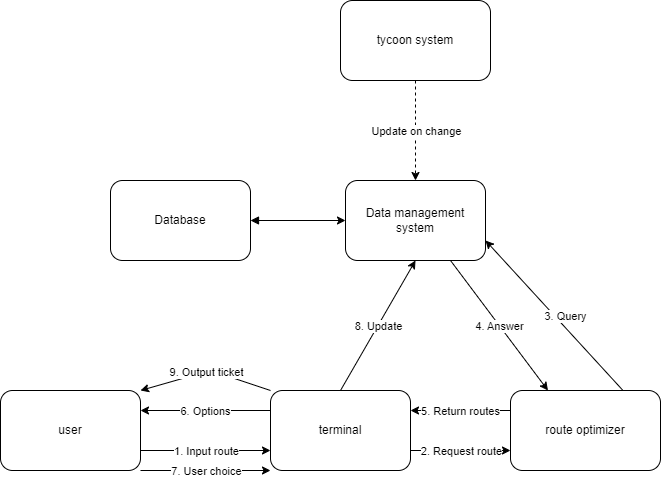
\includegraphics[width=\textwidth]{drawings/views_draft1/functional_view_draft1.png}
    \caption{Functional view model.}
    \label{fig:functional_view_model}
\end{figure}

\section*{Information Viewpoint}

\section*{Concurrency Viewpoint}

\section*{Development Viewpoint}

\section*{Deployment Viewpoint}